% !TeX TXS-program:compile = txs:///pdflatex/[--shell-escape]
\documentclass[12pt]{article}
\usepackage{times}\usepackage{setspace}\doublespacing\usepackage[margin=2.5cm]{geometry}
\usepackage{amsthm, amssymb}
\usepackage{bbold}
\usepackage{mathtools}
\usepackage[pdf]{graphviz}
\usepackage{listings}
\usepackage{caption}
\usepackage{url}
\usepackage{graphicx}      % for \includegraphics
\usepackage{fancyhdr}
\usepackage{titling}       % for \@title and \@author
% Paths and definitions
\graphicspath{{./images/}}
\newtheorem{definition}{Definition}

\title{Compilarea Rețelelor Petri: De la Descriere Formală la Simulare și Vizualizare}
\author{Mocanu Ștefan}

% Generează variabilele cu @
\makeatletter

\begin{document}

\begin{titlepage}

    % Redu marginile
    \newgeometry{left=2cm,right=2cm,bottom=1cm}
    
    \begin{figure}[!htb]
        \centering
        \begin{minipage}{0.2\textwidth}
            
\includegraphics[width=\linewidth]{logo-ub.png}
        \end{minipage}
        \begin{minipage}{0.5\textwidth}
            \large
            \vspace{0.2cm}
            \begin{center}
                \textbf{UNIVERSITATEA DIN BUCUREȘTI}
            \end{center}
            \vspace{0.3cm}
            \begin{center}
                \textbf{
                    FACULTATEA DE \\
                    MATEMATICĂ ȘI INFORMATICĂ
                }
            \end{center}
        \end{minipage}
        \begin{minipage}{0.2\textwidth}
            
\includegraphics[width=\linewidth]{logo-fmi.png}
        \end{minipage}
    \end{figure}
    
    \begin{center}
    \textbf{SPECIALIZAREA INFORMATICĂ}
    \end{center}
    
    \vspace{0.5cm}
    
    \begin{center}
    \Large \textbf{Lucrare de licență}
    \end{center}
    
    \begin{center}
    \huge \textbf{\MakeUppercase{\@title}}
    \end{center}
    
    \vspace{1cm}
    
    \begin{center}
    \large \textbf{Absolvent \\ \@author}
    \end{center}
    
    \vspace{0.25cm}
    
    \begin{center}
    \large \textbf{Coordonator științific \\ Lect.dr. Claudia-Elena Chiriță}
    \end{center}
    
    \vspace{2cm}
    
    \begin{center}
    \Large \textbf{București, iunie 2021}
    \end{center}
    \end{titlepage}
\restoregeometry
\newgeometry{
    margin=2.5cm
}

\cleardoublepage
% \phantomsection
% \addcontentsline{toc}{section}{Rezumat}
{\centering \section*{Rezumat} \par}

Acest proiect propune un instrument de tip linie de comandă pentru parsarea și simularea Petri Neturilor, cu suport pentru extensii precum tokenuri colorate, arce inhibitoare, constrângeri temporale și construcții high-level cu placeuri parametrizate. Creat în principal cu scop educațional pentru aprofundarea conceptelor de design al compilatoarelor și modelare formală, instrumentul transformă un limbaj specific într-o reprezentare internă, permițând simularea, generarea de cod și vizualizarea neturilor prin Graphviz. Deși nu include o interfață grafică și nu respectă complet standarde existente precum PNML, proiectul oferă o abordare flexibilă, bazată pe text, potrivită pentru experimente cu modele mari sau complexe. Posibile dezvoltări viitoare includ adăugarea unei interfețe grafice, îmbunătățirea semanticii rețelelor high-level și integrarea cu formate standard.

\bigskip

\bigskip

% \addcontentsline{toc}{section}{Abstract}
{\centering \section*{Abstract} \par}
This project presents a command-line tool for parsing and simulating Petri Nets, with support for various extensions such as colored tokens, inhibitor arcs, time constraints, and high-level constructs with parameterized places. Designed primarily for learning about compiler design and formal models, the tool translates a domain-specific language into an internal representation, allowing simulation, code generation, and visualization through Graphviz. While it lacks a graphical interface and full support for existing standards like PNML, the project offers a flexible, text-based approach suitable for experimenting with large or complex models. Potential future work includes adding graphical support, improving high-level net semantics, and integrating standard formats.

\tableofcontents
\newpage
\section{Introduction}
This thesis is both a research and software development project, situated at the intersection of the domains of Petri net theory and compiler design. It explores the use of formal methods for the modeling and simulation of concurrent systems, aiming to bridge the gap between theoretical models and executable implementations.

At the core of this work lies the general concept of Petri nets, a formal mathematical tool used to represent and analyze concurrent, distributed, and parallel systems. Petri nets model system behavior using a combination of places, transitions, and tokens, providing a framework for analyzing crucial system properties such as deadlocks, reachability, and synchronization. Their structured nature makes them especially useful for reasoning about complex system dynamics in a clear and analyzable way.

To support automated analysis and execution, this thesis integrates compiler techniques, highlighting the role of compilers in transforming high-level Petri net descriptions into executable code. By combining the rigor of Petri-net theory with the systematic transformation capabilities of compilers, this work proposes a domain-specific language that allows users to describe Petri nets in a structured and readable format. This language is then compiled into executable representations, facilitating the modeling, simulation, and visualization of concurrent systems.

The motivation behind choosing this topic stems from both a theoretical interest in formal systems and a practical desire to support verification and testing of concurrent and parallel systems. As distributed software becomes increasingly prevalent, tools that simplify the specification and analysis of such systems are of growing importance. A dedicated language for Petri nets supports this goal by lowering the barrier to entry for formal modeling and enhancing the efficiency of simulation and validation processes.

The main contribution of this thesis is the development of a domain-specific language for describing Petri nets, along with a compiler implemented in Haskell. This compiler translates Petri net descriptions into GoLang code for execution and GraphViz for graphical visualization, enabling both simulation and documentation. The project draws on knowledge from formal language theory, compiler construction, and concurrent system modeling, offering a cohesive and practical toolset for analyzing distributed behaviors.
    \subsection*{Why Petri Nets}
    One of the main motivations for choosing a project on Petri nets was my interest in distributed systems. These systems are inherently complex due to concurrency, synchronization, and communication challenges. Petri nets, with their formal semantics and graphical nature, provide a powerful framework for modeling and analyzing such systems. Their ability to represent parallelism and detect issues like deadlocks or race conditions makes them highly relevant for the study and simulation of distributed architectures.

    Additionally, at the time I selected this topic, I was curious about formal verification methods and wanted to explore how mathematical models could be used to reason about the correctness of systems. Petri nets offered an accessible and visually intuitive gateway into the world of formal methods. By working on this project, I was able to gain hands-on experience with the modeling and analysis of concurrent behavior, while also exploring how these models can be transformed into executable simulations, bridging the gap between theoretical models and practical implementations.

\section{Preliminaries}
    \subsection{Definitions}
    The following two definitions are from \cite{rozenberg1996elementary}:
    \begin{definition}
        A \textbf{net} is a triple \(N=(P,T,F)\) where: 
        \begin{enumerate}
            \item \(P\) and \(T\) are finite disjoint sets of \textbf{places} and \textbf{transitions}.
            \item \(F \subseteq (P \times T)\cup(T \times P)\) is a set of flow relations.
            \item for every \(t \in T\), there exists $p,q \in P$ such that $(p,t),(t,q) \in F$.
            \item for every $t \in T$ and $p,q \in P$, if $(p,t),(t,q) \in F$, then $p \neq q$.
        \end{enumerate}
    \end{definition}

    For a net \(N=(P,T,F)\) and \(t \in T\), we denote $\bullet t$ the incoming arcs into $t$ and $t \bullet$ the outcoming arcs from t. The notation is analogous for $p \in P$.

    \begin{definition}
        A \textbf{Petri net} is a net of the form $\mathrm{PN}=(N,M,W)$, where: 
        \begin{enumerate}
            \item $N=(P,T,F)$ is a net.
            \item \(M: P \rightarrow Z\) is a place multiset, where \(Z\) is a countable set. \(M\) maps for every place the number of tokens it has, and it is known as the \textbf{initial marking}, noted with \(M_0\) .
            \item \(W: F \rightarrow Z\) is an arc multiset, which denotes the arc's weight. 
        \end{enumerate}
    \end{definition}

    The following definition from \cite{diaz2013petri} describes the conditions for firing a transition, how a new marking $M'$ is created and what it is its relationship to the previous marking $M$.
    \begin{definition}
        Having a Petri net \(PN=(N,M,W)\) with \(N=(P,T,F)\):  
        \begin{enumerate}
            \item A transition \(t \in T\) can be \textbf{fired} if for every arc \(a=(p,t) \in \bullet t\), \(W(a) \le M(p)\).
            \item By firing t, a new marking $M'$ is created as follows: 
            \begin{displaymath}
                M'=\{(p,x)|\; p \in P,\; x = M(p) - W((p,t)) + W((t,p))\}
            \end{displaymath}
            If \((p,t)\notin T\) or \((t,p)\notin T\), then \(W(p,t)\), respectively \(W(t,p)\) will be subtituted with 0, or its equivalent in Z.
            \item If $M'$ can be obtained by firing a transition from $M$, then this relation is noted \(M \rightarrow M'\). 
            \item If $M'$ can be obtained by firing an arbitrary number of transitions starting with $M$, then $M'$ is reachable from $M$, and reachability is noted like this: \(M \xrightarrow{*} M'\).
        \end{enumerate}
    \end{definition}

    The following definition from \cite{girault2013petri} defines Coloured Petri Nets, which extend the definition of simple PN by allowing tokens to carry data values, called colours, enabling more compact and expressive models. Instead of using multiple places and transitions to represent different types of information or behavior, CPNs use colour sets and expressions to distinguish between token types and define complex conditions for transition firing. 
    \begin{definition}
        A \textbf{coloured Petri net (CPN)} is defined by a tuple \(\mathrm{CPN}=(N,C,M,W)\) where: 
        \begin{enumerate}
            \item $N=(P,T,F)$ is a net.
            \item \(C\) is the set of colour classes.
            \item \(M: P \rightarrow 2^{C \times Z}\) is the modified PN marking function to accomodate the use colours
            \item \(W: F \rightarrow 2^{C \times Z}\) is the modified PN arc weight function to accomodate the use of colours
        \end{enumerate}
    \end{definition}
    The following definition from \cite{diaz2013petri} introduces Petri Nets with inhibitor arcs, which extend the definition of simple PN by allowing transitions to be connected to places via inhibitor arcs. These arcs enable a transition to fire only when the connected place contains less tokens than them, allowing the modeling of non-monotonic behavior and enabling control based on the absence of conditions. This extension supports more expressive system descriptions, particularly for capturing mutual exclusion, conditional execution, and resource constraints in concurrent and distributed systems.
    \begin{definition}
        A \textbf{Petri net with inhibitor arcs} is defined by a tuple \(\mathrm{PNI}=(\mathrm{PN},\mathrm{Inh})\) where: 
        \begin{enumerate}
            \item \(PN\) is a Petri net using the above notation
            \item \(Inh\) is the inhibition matrix defined in \((Z_\omega \backslash 0)^{P\times T}\).
            \item To the firability criteria of a transition \(t \in T\) from a marking $M$, the condition of $M<Inh(t)$(the comparison is made component per component) is added.
        \end{enumerate}
    \end{definition}
    The following definition from \cite{diaz2013petri} presents Timed Petri Nets, which extend the definition of simple PN by associating time semantics with transitions or tokens. This addition enables the modeling of temporal constraints and delays in system behavior, allowing transitions to fire only after specific time intervals have elapsed. Timed Petri Nets are particularly useful for representing real-time systems, performance analysis, and scenarios where timing and synchronization are critical to system correctness.
    \begin{definition}
        Timed Petri nets extend Petri nets by associating a firing duration with each transition. More formally, a \textbf{timed Petri net} is a tuple $\mathrm{TPN}=(\mathrm{PN},\mathrm{IS})$, in which $\mathrm{PN}$ is a Petri net, and $\mathrm{IS}:T\rightarrow Q^+ \times (Q^+ \cup \{\infty\})$ is the static interval function. 
    \end{definition}
        
    The following definition from \cite{diaz2013petri} introduces \emph{High-Level Petri Nets}, a term we adopt to describe what are formally known as \emph{Parameterized Petri Nets}. These extend basic Petri nets by enabling parts of the net to be specified as parameterized templates. Such templates use indexed variables like \texttt{<N>} to define scalable sections that are automatically expanded into $N$ structurally identical subnetworks. Places, transitions, and arcs involving these parameters are replicated per instance, allowing concise modeling of systems with repeating components such as multiple clients or concurrent processes. This approach supports modular design and simplifies the specification of large, regular Petri nets.
    \begin{definition}
        A \emph{parameterized Petri net (PPN)} is a tuple
\[
\mathrm{PPN} = (P_0, P_{\mathrm{tmpl}}, T_0, T_{\mathrm{tmpl}}, F, M_0)
\]
where:
\begin{itemize}
    \item $P_0$ and $T_0$ are sets of base places and transitions.
    \item $P_{\mathrm{tmpl}}$ and $T_{\mathrm{tmpl}}$ are sets of place and transition templates.
    \item $F \subseteq (P_0 \cup P_{\mathrm{tmpl}}) \times (T_0 \cup T_{\mathrm{tmpl}})$ is the arc set.
    \item $M_0 : P_0 \cup P_{\mathrm{tmpl}} \to \mathbb{N}$ is the initial marking.
\end{itemize}

Given a replication factor $N \in \mathbb{N}_{>0}$, the unfolded net $\mathrm{PPN}(N)$ is a standard Petri net where each $p \in P_{\mathrm{tmpl}}$ and $t \in T_{\mathrm{tmpl}}$ is instantiated as $p_1, \dots, p_N$ and $t_1, \dots, t_N$.

The flow relation and initial marking are lifted accordingly. For example, $(p, t) \in F$ with $p, t$ both templates expands to $(p_i, t_i)$ for all $i$.

    \end{definition}


    \subsection{Current State of Petri Net Modeling}

        \subsubsection{Petri Net Markup Language (PNML)}

        The \textit{Petri Net Markup Language} (PNML) was introduced as an attempt to standardize the representation of Petri Nets in a structured, tool-independent way. As described by Weber and Kindler~\cite{weber2003petri}, PNML defines an XML-based format designed to encode various classes of Petri Nets, including Place/Transition nets, Colored Petri Nets, and more. It aims to facilitate tool interoperability and model exchange between different Petri Net applications and environments.

        To date, PNML remains the closest the Petri Net research community has to a widely accepted standard for representing and exchanging Petri Net models. Its structure allows for extensibility and is supported by several modeling tools and academic frameworks. However, due to the complexity and verbosity inherent in XML, human readability and direct manipulation are often limited without dedicated graphical interfaces or tool support.

        \subsubsection{Existing Tools and Modeling Platforms}

        Numerous tools exist for modeling, simulating, and analyzing Petri Nets. Notable platforms include:

        \begin{itemize}
            \item \textbf{CPN Tools} \cite{verbeek2021cpn} is a widely-used environment for Colored Petri Nets. It supports graphical modeling and powerful simulation capabilities tailored to high-level Petri Nets.
            \item \textbf{Petrinet Editor} \cite{app10217662} offers a browser-based modeling interface for basic and extended Petri Net types, with export and visualization support.
            \item A comprehensive and regularly updated list of Petri Net tools is maintained by the University of Hamburg~\cite{tgi_petri_tools}. This database includes editors, analyzers, simulators, and verification tools for a wide spectrum of Petri Net variants.
        \end{itemize}

        Despite the variety of existing solutions, many tools target specific net types or modeling scenarios and may lack support for extensible, user-defined features such as parametric expansion, custom net transformations, or integration into modern language tooling (e.g., JSON, Graphviz, or Go code generation). These gaps motivate further exploration into new modeling approaches and DSLs tailored for flexible and composable Petri Net representations.


    \subsection{Objectives of the Thesis in Context}
    The main goal of this thesis is to develop a domain-specific language for defining Petri nets, along with a compiler that translates these definitions into executable code for simulation and LaTeX code for visualization. The specific objectives are:
    \begin{itemize}
        \item To design a simple and expressive language for defining Petri nets.
        \item To implement a compiler in Haskell that generates both simulation-ready code and graphical representations.
        \item To compare this approach with existing tools and evaluate its advantages in terms of usability, automation, and flexibility.
    \end{itemize}
    This project bridges the gap between formal modeling and implementation, aiming to make Petri Net analysis not only more accessible but also automated.
    
\section{Petri Net Description Language}
    We start a few preliminary notions on the compilation in Haskell, a short presentation motivation the usage of the programming language Go.
    Then we describe how the DSL of this thesis was defined and how it was implemeted and tested.
    \subsection{Compilation in Haskell}
        \begin{definition}
            A compiler is a program that translates source code written in one language into another form, typically a lower-level language.
        \end{definition}
        Compilers are usually confused with transpilers or interpreters. 
        The main difference between a compiler and a transpiler is that the former translates source code from one language to another without lowering the abstraction level, whilst the first one usually lowers the abstraction level. An example of the usage of transpilers is related to TypeScript language which is a superscript of JavaScript.
        The difference between a compiler and an interpreter consists in the time at witch the translation is done. In the case of a compiler, the translation is done prior to execution, while in the case of an interpreter, the code is translated line by line at runtime. For instance, interpreters are used for the Python programming language, and Java has a compiler-interpreter hybrid.
        \cite{alfred2007compilers}
        \begin{definition}
            Syntactic analysis, or parsing, is the compiling phase that processes a sequence of tokens (usually from the lexical analyzer) and produces a structured representation—often an abstract syntax tree (AST)—based on the grammar of the source language.
        \end{definition}
        
        Traditionally, syntactic analysis is performed using classical parsers, such as top-down (LL) or bottom-up (LR, LALR) algorithms. These parsers are typically generated by tools like Yacc or Bison, based on a formal grammar written in a declarative notation such as BNF. The grammar is separated from the implementation, and the process often requires an accompanying lexer (e.g., Flex) to provide tokens.
        \cite{alfred2007compilers}

        In contrast, parser combinators \cite{hutton1996monadic} offer a more modern and expressive approach, especially in functional programming languages like Haskell. A parser combinator library allows the programmer to define parsers directly in code, using higher-order functions to build complex parsers from simpler ones. This eliminates the need for external grammar files and generation steps. In Haskell, the most widely used library for this purpose is Parsec \cite{parsec}.
        
        Parsec allows grammars to be embedded directly into Haskell source code, making the syntax of the language itself a first-class citizen. This style supports powerful abstraction, composability, and precise error handling, as each parser is a value and can be passed around, combined, or reused. Furthermore, it enables fine-grained control over the parsing process, and benefits from Haskell's strong static type system.
        
        In this project, the syntax of the Petri Net description language is implemented using Parsec. The choice of Parsec over a traditional parser generator was motivated by its flexibility and seamless integration with Haskell's data structures. The custom language that we define supports advanced constructs, such as parametrized high-level net sections, which can be naturally represented and parsed using Parsec's compositional design.
        
    \subsection{GoLang}
    Go (or Golang) \cite{golang} is a statically typed, compiled programming language developed at Google, designed for simplicity, performance, and concurrency, as discussed by Pike \cite{pike2012go}. Its usage in this project is motivated by several key features that align well with the requirements of simulating and executing Petri nets.

    Firstly, Go offers native support for concurrency through \emph{goroutines} and \emph{channels} \cite{pike2012go}. Since Petri nets are inherently concurrent models, simulating them efficiently requires lightweight thread-like constructs and synchronization mechanisms. Go's model of concurrent execution, inspired by Hoare's Communicating Sequential Processes (CSP) \cite{brookes1984theory}, maps naturally to the semantics of Petri nets, making the implementation of concurrent behavior both elegant and efficient.
    Even though I did not use this feature of the language in the project, it can be extended in the future to include features that would benefit from it, like cicle detection, or the firing of multiple independent transitions at once.

    Secondly, Go has a minimalistic and clean syntax, which improves readability and maintainability. For a simulation backend intended to be easily extensible and understandable, avoiding the complexity of languages like C++ or Java is a significant benefit. Furthermore, the absence of a complicated type system or inheritance hierarchy in Go simplifies the representation of tokens, transitions, and execution logic.

    Thirdly, Go produces statically linked, self-contained binaries, facilitating easy deployment of the simulation tool without runtime dependencies \cite{pike2012go}. This makes it ideal for building tools that are meant to be used in varied environments, especially in academic or distributed computing setups where installation overhead should be minimal.

    Lastly, Go has a growing ecosystem and active community, with tools for performance profiling, testing, and package management. It is increasingly used in systems programming, making it a pragmatic choice that balances low-level control with developer productivity.

    In conclusion, Go's design principles, concurrency model, ease of deployment, and simplicity make it particularly well-suited for the execution layer of a Petri net simulation system. These factors justify its selection over alternatives such as Python (limited concurrency performance), Java (heavier runtime), or C++ (steeper learning curve and more complex concurrency primitives).

    \subsection{Implementation}
        \subsubsection{The PNDL Language}
            To support the modeling of various types of Petri Nets in a flexible and extensible way, I designed a custom domain-specific language called \emph{Petri Net Description Language} (PNDL). This language is used to define Petri Nets in a human-readable and modular format, supporting extensions such as colored tokens, timing constraints, inhibitor arcs, and high-level parameterized components. The syntax of PNDL is intentionally minimal and declarative, using sections like \texttt{NET\_TYPE}, \texttt{VARIABLES}, \texttt{PLACES}, \texttt{TRANSITIONS}, and \texttt{ARCS} to describe the structure and behavior of the net. 
            Figure~\ref{fig:PNDLsyntax} in the Appendix presents the core syntax of PNDL, along with inline comments that clarify the semantics and conditional requirements for each section based on the net type. This format serves as the input to the compiler I developed, which translates PNDL specifications into JSON and Graphviz representations.      
        \subsubsection{The Interface of the Project}   
            The final implementation of the parser program has a CLI. The interface has three commands: \texttt{compile}, \texttt{generate-go} and \texttt{graphviz}. Every command takes as argument a file written in the format described in the next subsections. In the further sections of this chapter, the behavior and implementation details will be described.

        \subsubsection{Compile command}
        To interpret a PNDL file, the \texttt{compile} command invokes a series of functions that parse its contents using the \texttt{Parsec} module. These functions structure the parsed data into custom Haskell objects, which are then translated into JSON, depending on the type of Petri Net being described. The compilation process supports several Petri Net extensions, as follows:

        \begin{enumerate}
            \item \textbf{Simple Petri Nets:}
            \begin{itemize}
                \item The initial marking is stored in a dedicated object that maps each place name to its corresponding token count in $M_0$.
                \item Each place is represented by an object containing a placeholder attribute, allowing future extensions such as dynamic modification of the place structure.
                \item Arcs are grouped by transition and direction (input or output). Each arc includes a \texttt{weight} attribute.
            \end{itemize}
        
            \item \textbf{Coloured Petri Nets:}
            \begin{itemize}
                \item Token counts and arc weights are represented as maps from color names represented strings to integer values, instead of plain integers.
            \end{itemize}
        
            \item \textbf{Timed Petri Nets:}
            \begin{itemize}
                \item Each transition object includes two additional integer attributes: \texttt{minTime} and \texttt{maxTime}, defining the transition's firing interval.
            \end{itemize}
        
            \item \textbf{Inhibited Petri Nets:}
            \begin{itemize}
                \item Transitions may optionally include an \texttt{inh} attribute for inhibitor arcs. This attribute is an integer for simple nets, or a color-to-count map for coloured nets.
            \end{itemize}
        
            \item \textbf{High-Level Petri Nets:}
            \begin{itemize}
                \item Places defined with a parameter (e.g., \texttt{Place<N>}) are expanded into multiple concrete places: \texttt{Place\_1}, \texttt{Place\_2}, \dots, \texttt{Place\_N}, each initialized with the same token values.
                \item Each generated place \texttt{Place\_X} includes an entry in the initial marking such as \texttt{\{Variable\_X: 1\}}. For non-coloured nets, all tokens are tagged with a default color: \texttt{token}.
                \item Transitions that are not connected to high-level places are replicated for every combination of parameter values. For every variable $V$, this results in transitions like:
                \[
                    T\_V\_1, \quad T\_V\_2, \quad \dots, \quad T\_V\_n
                \]
                \item Transitions that connect to high-level places are only expanded based on the variables associated with those specific places.
                \item Each generated transition \texttt{T\_Vx\_y} has an entry \texttt{\{Vx\_y: 1\}} added to every weight map in its arcs, indicating the specific instance it operates on.
                \item All transformations related to high-level Petri Nets are performed entirely at compile-time. The resulting JSON, and subsequently the Go code, treats the net as if it were a simple, non-parametrized Petri Net.
            \end{itemize}
        \end{enumerate}
        \subsubsection{Generate-Go commnand}
            The \texttt{generate-go} command interprets only the \texttt{NET\_TYPE} directive from the PNDL file and produces a fully functional Go source file based on a predefined template. This template is almost identical to a standard Go file, with the exception of custom compile-time conditionals expressed using the syntax \texttt{<<condition, code>>}. These conditional code blocks are evaluated during generation and are only included in the final output if their corresponding condition holds. Conditions can be logical combinations such as \texttt{COLORED}, \texttt{NOT COLORED}, \texttt{TIMED}, \texttt{INHIBITED}, or even composite conditions like \texttt{TIMED AND INHIBITED}.

            The structure of the generated Go file is modular and follows the logic of simulating a Petri Net execution:
            
            \begin{itemize}
            \item The \textbf{data types} (\texttt{Arc}, \texttt{Transition}, \texttt{Marking}, \texttt{Net}, and \texttt{JSONInput}) are defined first. These types adapt to the net type using the conditional syntax. For example, in a COLORED net, arc weights and initial markings are maps from color names to integers, while in a simple net, they are plain integers.
            \item The \textbf{JSON loader} reads the net structure and initial marking from \texttt{net.json}, processes the color set (if applicable), and fills in any missing places with zero tokens. For TIMED nets, default firing intervals are ensured to be at least 1 if not explicitly set.

            \item The \textbf{arc comparison function} (\texttt{compareArc}) evaluates whether a transition is enabled by comparing the current marking with the arc’s weight and inhibitor values. Different versions of this logic are compiled depending on the combination of COLORED and INHIBITED settings.

            \item The \textbf{main simulation loop} repeatedly computes the set of viable transitions, selects one randomly, and fires it. For TIMED nets, the logic becomes more complex: transitions are started and appended to an \texttt{activeTransitions} list, which tracks remaining execution time. When a transition’s timer expires, its output arcs are applied.

            \item The simulation continues until no more transitions are viable and no timed transitions are pending (in TIMED mode).

            \item Additional helper functions handle tasks such as transition selection, applying input/output arcs, and managing time progression.
            \end{itemize}

            All code variants are embedded in the template using the \texttt{<<condition, code>>} syntax. During generation, the system performs a textual transformation, resolving all such blocks based on the current Petri Net type. This ensures that the final Go program is minimal, readable, and free of unused logic paths.
        
        
        \subsubsection{GraphViz Generation}
            GraphViz is a graph visualization tool written in dot syntax, that can be easily compiled in a LaTeX environment. This representation can be exported in all sorts of formats like PDF, PNG, JPEG and many more.  

            The GraphViz module of the project is responsible for producing a .dot representation of a Petri Net. Its modus operandi closely mirrors that of the \texttt{toJSON} Parsec-based parser. It also relies on a Parsec parser to interpret the PNDL input and generate the corresponding arguments for the \texttt{DOT} syntax. The structure of the parser and its logic for handling \texttt{COLORED}, \texttt{TIMED}, and \texttt{INHIBITED} nets are analogous to those used in the JSON generator.
            
            The key distinction arises when dealing with \texttt{HIGH-LEVEL} nets. In this case, high-level constructs such as variable-bound places and transitions are not expanded into all possible concrete instances. Instead, they are grouped according to the variable on which they depend. Each such group is rendered as a distinct subgraph (or \texttt{subgraph cluster}) within the overall DOT graph. This visual separation serves to highlight the parametric nature of the net and the dependencies of each group on its associated variable.
            
            All remaining non-parametric (simple) places and transitions are placed in a special group labeled \texttt{simple}, representing components independent of any variable. This structured organization enhances readability and provides insight into the modular, parameterized design of high-level nets.

            In the generated GraphViz graph, places and transitions are visually distinguished using different node formatting styles. Places are represented as ellipses, while transitions are drawn as rectangles. This differentiation aligns with common Petri Net visualization conventions and improves the interpretability of the diagram.
    
        \subsection{Comparison with Existing Tools}

            The domain of Petri Net modeling has seen the development of various tools and standardization efforts. Among these, the \emph{Petri Net Markup Language (PNML)}~\cite{weber2003petri} represents the most widely accepted attempt at a standardized representation format. PNML is designed for interoperability and exchange of models between tools, but its XML-based structure can become verbose and less suitable for fast prototyping.
            
            Graphical modeling environments such as \emph{CPN IDE}~\cite{verbeek2021cpn} and \emph{PetriNet Editor}~\cite{app10217662} offer visual construction, simulation, and in some cases, code generation capabilities. These tools focus on ease of use for system designers and support a wide range of Petri Net extensions. Additionally, the \emph{Petri Nets Tools Database}~\cite{tgi_petri_tools} catalogs a wide variety of tools supporting analysis, modeling, and transformation of Petri Nets.
            
            In contrast, the project presented in this thesis introduces a textual, compiler-inspired pipeline for modeling Petri Nets. One of its main contributions is a high-level modeling mechanism that supports \emph{parameterized nets}, allowing users to define templates with indexed variables. This supports concise descriptions of structurally repetitive systems, improving scalability and modularity. Unlike CPN IDE or PetriNet Editor, which support simulation and GUI modeling, this tool is optimized for textual specification, batch processing, and automatic code generation.
            
            Furthermore, the tool integrates support for extensions such as \emph{Colored}, \emph{Timed}, and \emph{Inhibited} Petri Nets within a unified syntax. This composability is particularly useful in automated or programmatic settings. However, it currently lacks several features provided by mature tools:
            \begin{itemize}
                \item Only textual simulation is supported via the Go backend; lacks visual or interactive analysis tools.
                \item There is no graphical modeling interface, which may hinder adoption by users unfamiliar with textual DSLs.
                \item It does not support PNML import/export, limiting interoperability with standardized ecosystems.
            \end{itemize}
            
            Despite these limitations, the tool excels in structural scalability and automation. It is particularly well-suited for use cases involving programmatically generated models, code integration, or parameter sweeps, and thus serves as a complementary approach to existing GUI-based and simulation-focused tools.
    \subsection{Testing the Project with Examples}
        \subsubsection{Inhibited Arcs}
            Listing~\ref{fig:example2code} in the Appendix describes a net with an inhibited arc. Its graph is shown in Figure~\ref{fig:example2png}, demonstrating that the GraphViz output can support this type of arcs. In Figure~\ref{fig:example2output}, the steps of the execution of the net can be seen. We can observe how the program stops when the \texttt{Consumer} place has 5 tokens. 
        \subsubsection{Coloured tokens}
            Listing~\ref{fig:example3code} describes the same net as before but has coloured tokens. It consumes blue and yellow tokens and produces green tokens, as seen in Figure~\ref{fig:example3png}. The output stops when the consumer has 5 green tokens, as seen in Figure~\ref{fig:example3output}.
        \subsubsection{Timed transitions}
            Listing~\ref{fig:example4code} describes the same net as before but has timed transitions. This feature does not impact the GraphViz output. When running the generated GoLang code, an output similar to Listing~\ref{fig:example4output} is generated. The output can only be similar because Timed Nets introduce a randomised element, the duration of the transitions. 
        \subsubsection{Highlevel nets}
            Listing~\ref{fig:limit1} describes a high level net, with the difference that here $N$ is instanciated as $100$. Because a highlevel net does not change the behavior of the GoLang code, its output isn't included. In contrast, the GraphViz representation of this net has a major difference from the above discussed representations, and can be seen in Figure~\ref{fig:example1png}. That difference is the presence of the gray rectangle surrounding the places and transitions that depend on the variable $N$.  
    \subsection{Testing the Limits of the Tool}   
        To explore the performance boundaries and correctness of the Petri Net toolchain, a series of stress tests were designed and executed. These tests targeted both the parser and the backend code generation components.
        \subsubsection{Parametrized Expansion Overhead}
            One approach for evaluating scalability involves defining a \textbf{High-Level Petri Net} with an extremely large parameter. The network described in Listing~\ref{fig:limit1} models a client-server interaction, parameterized over $N = 1{,}000{,}000$ clients, and incorporates \texttt{TIMED}, \texttt{INHIBITED}, \texttt{COLORED}, and \texttt{HIGH\_LEVEL} features.

            Execution of this definition resulted in the operating system terminating the process due to excessive memory consumption or CPU overload. This indicates that the tool currently encounters performance bottlenecks when expanding high-cardinality parametrized definitions. The corresponding error is shown in Figure~\ref{fig:error}. The exact value of $N$ that triggers this error varies depending on the machine's hardware specifications. In the case of my machine which had around 11.5 free GiB of RAM, the problems started showing up for $N > 700{,}000$

        \subsubsection{Integer Overflow in Go Backend}
            A separate test focused on identifying numeric limitations in the backend code generation. The network described in Listing~\ref{fig:limit2} utilizes large token weights to provoke overflow behavior in the Go language implementation.

            This net successfully compiles and passes through the parser. However, execution of the generated Go code results in overflow, as the default integer type on the target system is a 64-bit signed integer, with a maximum representable value of $2^{63} - 1$. This exposes a limitation in the type safety of the backend generator and suggests a need for improved handling of numeric ranges.

            Figure~\ref{fig:markings} shows the behaviors of the Go script for the first 10 iterations (plus the starting marking) of the net. We can observe how the places sometimes have negative values, a clear sign of integer overflow.


\section{Conclusion}
    \addcontentsline{toc}{subsection}{Shortcomings of the Project}
    \subsection*{Shortcomings of the Project}

    This project, while functional in its core objectives, has several limitations when compared to existing tools in the domain.

    \subsubsection*{Missing Features Present in Other Tools}

        A number of features commonly found in similar tools are not implemented in this project:
        \begin{itemize}
            \item \textbf{Graphical Interface}: The tool lacks a graphical editor or visualization interface, unlike tools such as CPN Tools~\cite{verbeek2021cpn} or PetriNet Editor~\cite{app10217662}. This omission stems from the project's primary goal: learning about compiler construction and language design. As such, efforts were focused on parsing, representation, and code generation rather than UI development.
            \item \textbf{Standard Integration}: The tool does not natively support the Petri Net Markup Language (PNML)~\cite{weber2003petri}, which is widely regarded as a standard. This was largely due to late discovery of the format during the development process. A future version of the project could integrate support for PNML import/export to improve interoperability.
        \end{itemize}

    \subsubsection*{Limitations in the High-Level Net Implementation}

        The high-level Petri Net implementation introduces several structural restrictions:

        \begin{itemize}
            \item \textbf{No Cross-Instance Arcs}: The tool does not support transitions connecting instances of different indices in high-level places. For example, a transition with an incoming arc from \texttt{P<i>} and an outgoing arc to \texttt{P<j>} (where $i \ne j$) is disallowed, due to the logic used in the unfolding process.
            \item \textbf{Uniform Initial Marking}: All instances of a high-level place \texttt{P<N>} must have the same initial marking. It is not possible to specify distinct initial token distributions for different values of $i$ within the same parameterized place.
            \item When more than one group of high-level places interacts within the same net, the resulting behaviour becomes undefined. The current expansion logic does not resolve interactions across distinct parameter groups, leading to uncertain semantics.
        \end{itemize}

    % \subsubsection*{Future Work}

    % Despite these shortcomings, the project lays a foundation that can be improved upon. Future revisions could address these limitations by:
    % \begin{itemize}
    %     \item Adding PNML compatibility and GUI support.
    %     \item Refining the unfolding logic to allow cross-instance arcs.
    %     \item Supporting non-uniform initial markings for parameterized places.
    % \end{itemize}

    % There is clear potential for future work to make the tool more competitive with existing platforms, while retaining its compiler-oriented design philosophy.
\addcontentsline{toc}{subsection}{Overview and Future Work}
\subsection*{Overview and Future Work}
The development of this project was driven by a desire to explore compiler design principles through the lens of a domain-specific language for modeling Petri Nets. The goal was to support advanced features such as high-level constructs, colored tokens, timed behavior, and inhibitor arcs, and to compile these into executable code and visualization formats. The implementation focused on correctness and extensibility, with an emphasis on the backend logic rather than user interface aspects.

Future improvements could include the development of a graphical user interface (GUI), support for simulation interactivity, formal verification tools, and alignment with existing standards such as the Petri Net Markup Language (PNML). Additionally, addressing current limitations of high-level net support, such as interactions between multiple parameterized groups, could significantly enhance the tool's expressiveness and reliability.

From a personal standpoint, this project provided valuable insight into language parsing, transformation pipelines, and system modeling. The results achieved are significant in that they enable efficient modeling of complex systems using a concise and modular syntax. While not aiming to compete directly with mature tools in the field, this project represents a meaningful proof of concept and an educational endeavor with tangible outcomes.

In terms of practical applications, the tool can be used in academic environments for teaching formal methods or as a lightweight modeling solution for prototyping concurrent systems. With continued development, it has the potential to serve as a flexible framework for Petri Net analysis in specialized domains such as distributed systems, protocol verification, or embedded systems design.

\newpage

\bibliographystyle{IEEEtran}
\bibliography{citations}
\newpage
\addcontentsline{toc}{section}{Appendix}
\section*{Appendix}
    \begin{figure}[hbtp]
        \caption{PNDL syntax}
        \label{fig:PNDLsyntax}
        \begin{lstlisting}[language=C,frame=single]
~NET_TYPE
COLORED | TIMED | INHIBITED | HIGH_LEVEL   
// Specify one or more net extensions
// If the net is simple, this section can be ommited

~VARIABLES
VariableName = Value                                 
// Optional variables used for parametrization
// If the net is not high level, this section can be ommited

~PLACES
PlaceName[<Variable>] [tokens={color1:count, color2:count, ...}]
// For coloured nets
PlaceName[<Variable>] [tokens=count]
// For simple nets
// Tokens field is optional
// In its absence, the m0 will be filled with 0

~TRANSITIONS
TransitionName [time=(min,max)]                      
// Optional time interval for timed nets
// If absent, then time will default to (1,1), for timed nets

~ARCS
Source -> Target [weight=value] [inh=value]
// Only one of source or target can be a place
// Only one of source or target can be a transition
// If source is a transition, then the arc is an output of Source
// If Target is a transition, then the arc is an input of Target
// The weight field is always present
// Value can be replaced with an integer or a color-value map
// The inh field is ommited if the net doesn't have inhibitor arcs
// If the net has inhibitor arcs this field is optional
// If Source or Target is a high level place then 
//the <Variable> of the place needs to be present
        \end{lstlisting}
    \end{figure}
    \lstset{
        breaklines=true,
        basicstyle=\ttfamily\small,
        frame=single,
        captionpos=b
      }
      
    \begin{figure}[p]  % [p] for page of floats
        \centering
        \lstinputlisting[caption={Code generating memory errors}, label={fig:limit1}]{limit1.txt}
    \end{figure}

    \begin{figure}[htbp]
        \centering
        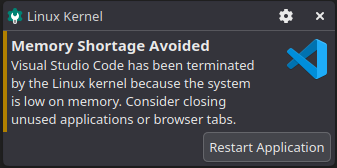
\includegraphics[width=\linewidth/2]{Error_message.png}  % adjust width as needed
        \caption{The error message}
        \label{fig:error}
    \end{figure}
      
    \begin{figure}[p]  % [p] for page of floats
        \centering
        \lstinputlisting[caption={Code generating memory errors}, label={fig:limit2}]{limit2.txt}
    \end{figure}

    \begin{figure}[htbp]
        \centering
        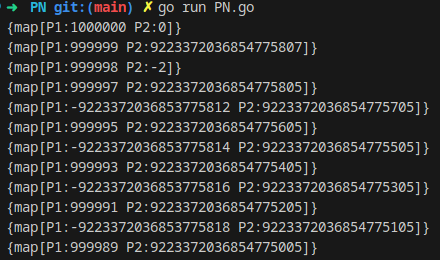
\includegraphics[width=\linewidth/3 *2]{Marking.png}  % adjust width as needed
        \caption{The generated markings by the net in Listing~\ref{fig:limit2}}
        \label{fig:markings}
    \end{figure}

    \begin{figure}[p]  % [p] for page of floats
        \centering
        \lstinputlisting[caption={Code testing inhibitor arcs}, label={fig:example2code}]{example2.pndl}
    \end{figure}

    \begin{figure}[htbp]
        \centering
        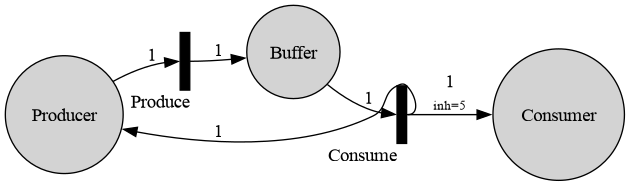
\includegraphics[width=\linewidth]{example2.png}  % adjust width as needed
        \caption{The generated net in Listing~\ref{fig:example2code}}
        \label{fig:example2png}
    \end{figure}

    \begin{figure}[htbp]
        \centering
        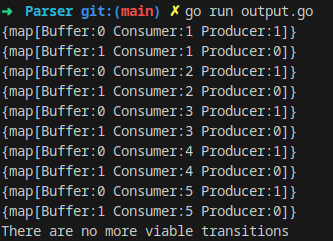
\includegraphics[width=\linewidth/2]{Output2.png}  % adjust width as needed
        \caption{The generated output for the net in Listing~\ref{fig:example2code}}
        \label{fig:example2output}
    \end{figure}

    \begin{figure}[p]  % [p] for page of floats
        \centering
        \lstinputlisting[caption={Code testing inhibitor arcs with coloured tokens.}, label={fig:example3code}]{example3.pndl}
    \end{figure}

    \begin{figure}[htbp]
        \centering
        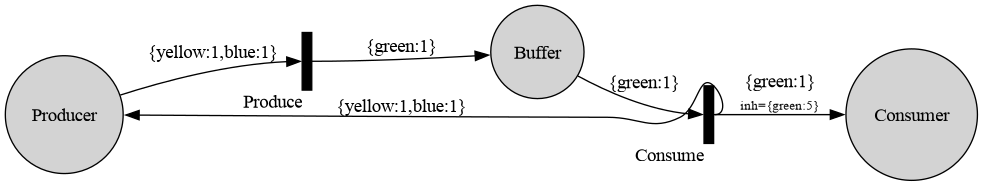
\includegraphics[width=\linewidth]{example3.png}  % adjust width as needed
        \caption{The generated net in Listing~\ref{fig:example3code}}
        \label{fig:example3png}
    \end{figure}

    \begin{figure}[htbp]
        \centering
        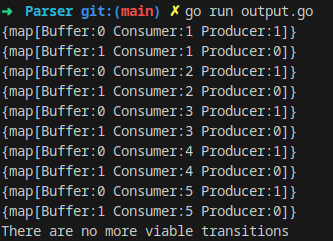
\includegraphics[width=\linewidth/2]{Output2.png}  % adjust width as needed
        \caption{The generated output for the net in Listing~\ref{fig:example3code}}
        \label{fig:example3output}
    \end{figure}

    \begin{figure}[p]  % [p] for page of floats
        \centering
        \lstinputlisting[caption={Code testing inhibitor arcs with coloured tokens and timed transitions.}, label={fig:example4code}]{example4.pndl}
    \end{figure}

    \lstinputlisting[
        caption={Output resulting from running the net from Listing~\ref{fig:example4code}},
        label={fig:example4output},
        breaklines=true,
        basicstyle=\ttfamily\small,
        frame=single,
        captionpos=b
    ]{Output4.txt}
    \begin{figure}[htbp]
        \centering
        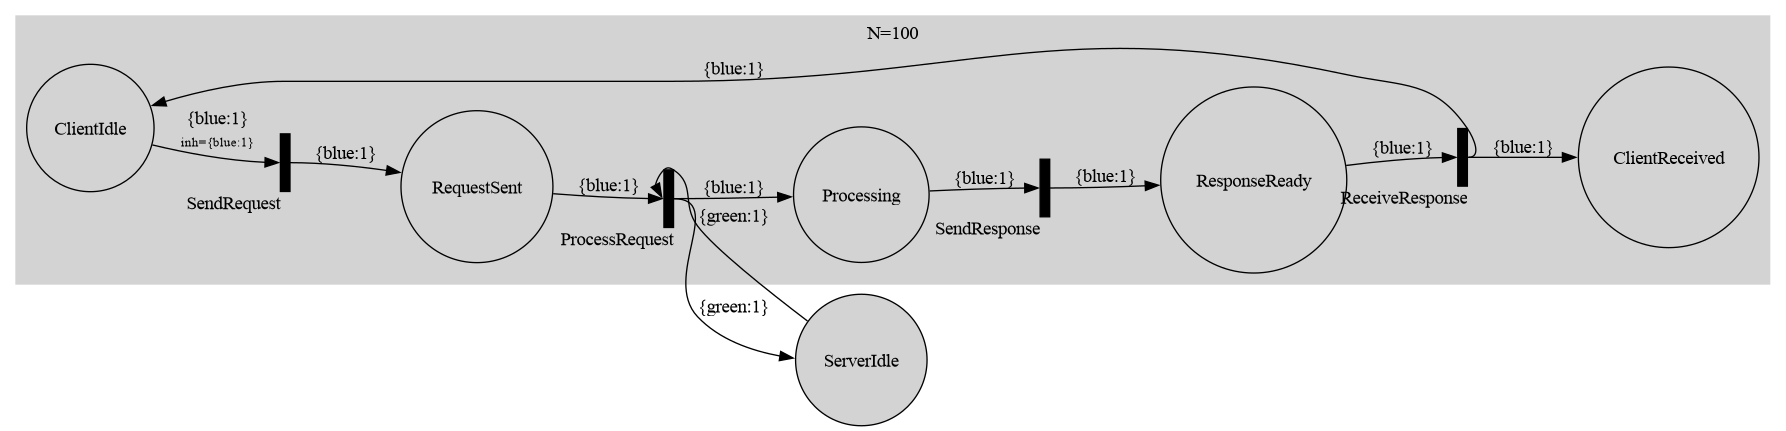
\includegraphics[width=\linewidth]{example1.png}  % adjust width as needed
        \caption{The generated net in Listing~\ref{fig:limit1}}
        \label{fig:example1png}
      \end{figure}
\end{document}
